\documentclass{ds-report} 
\usepackage{babel}[dutch]
\usepackage{graphicx}

\assignment{Project} % Set to `Remote communication` or `Project`.
\authorOne{Martijn Leplae} % Name of first team partner.
\studentnumberOne{r0737706} % Student number of first team partner.
\authorTwo{Andreas Hinderyckx} % Name of second team partner.
\studentnumberTwo{r0760777}  % Student number of second team partner.

\begin{document}
	\maketitle

	\paragraph{Question 1}
	The component diagram can be found as figure \ref{fig:component}. We show every component in a `component'-box, along with relevant class objects in yellow boxes. The half open circles and full circle arrows indicate required and offered interfaces respectively.
	
	The front-end exists of the computer of the customer, which can be seen on the left hand side of the diagram. The back end consists of the Google cloud platform on one hand, and the Theatre servers on the other hand.
	\paragraph{Question 2} 
	We've made use of the Spring boot API to be able to simply create an endpoint te receive the messages of our Google Pub/Sub implementation. For this scenario, we could simply add the \texttt{@RestController} annotation and provide the code which corresponds to this endpoint. The specific behaviour of receiving POST-requests can then be added by providing the method with an \texttt{@PostMapping} annotation.
	
	The addition of Pub Sub API hides the complexity of implementing a subscription service for clients to subscribe to certain topics. 
	
	\paragraph{Question 3} 
	In the method that confirms requested quotes (i.e. transforms them into bookings), we've made use of the Pub/Sub API to make the process of a client requesting a booking and the server confirming it asynchronous. 
	
	The steps that occur in the indirect communication are:
	 \begin{itemize}
	 	\item The channel of the project, \texttt{Topic} and \texttt{PubSubMessages} instances are created,
	 	\item Create a \texttt{Publisher} which publishes \texttt{PubsubMessage}s for a given \texttt{Topic} on the channel created above.
	 	\item The message containing the quotes to be booked and required attributes are serialized and sent over the channel by the publisher as a \texttt{PubsubMessage}.
	 	\item Next, on the subscriber side, at our custom endpoint, the messages are received and unmarshalled and parsed into its original form.
	 	\item Finally, a PUT request is performed for each quote to confirm its corresponding booking on the theater company server.
	 \end{itemize}
 
 	\paragraph{Question 4}
 	Taking our endpoint created in function of the Pub/Sub mechanism as background worker, the marshalled form of the list of quotes to be booked is passed, along with other required parameters to perform the PUT-request: the API key and the name of the customer who makes the bookings. 
 	
 	If the server were physically separate machine, it wouldn't be able to make a reference to the object of the client. Therefore, it makes sense to marshall a copy of the quotes and send this to the server side such that it has its own local copy to work with.
	
	\paragraph{Question 5}
	For our small scale application, the indirect communication (Pub/Sub) only introduces some extra delay when confirming a booking due to the asynchronous nature of Pub/Sub. This implementation becomes advantageous, however, when scaling the application to a larger scenario. Then a large amount of applications or clients can all make use of the same Pub/Sub server, subscribers can easily filter out the messages they want to receive out of a common channel these are sent over.
	
	\paragraph{Question 6}
	As mentioned above, for small scale scenarios such as that of our application, the client only perceives increased delay due to the asynchrony introduced by Pub/Sub.
	
	\paragraph{Question 7}
	It should not be possible to perform a double booking with our implementation. Our approach is as follows: when a client wants to make a series of bookings, these are stored in a list and sequentially placed in a PUT request to try to obtain the corresponding ticket. As soon as one of these quotes can't be booked, the entire list of tickets conform to the requested bookings is deleted with a corresponding DELETE-request. As we are allowed to assume that these DELETE-requests are fully reliable and the company is assumed to be reliable as well --- as mentioned in the assignment --- this approach ensures that only the client who books his ticket first can obtain it: any other client trying to obtain the same ticket afterwards, will receive an error in the PUT request and thus will have its requested tickets removed from the server.
	
	\paragraph{Question 8} 
	Suppose there are multiple groups of people where each group has a different list of permissions. If we were to store a list of people who are allowed to perform a certain task and were to do this for each task, it would quickly become cumbersome to check whether a certain user is allowed to perform a certain task. Analogously, if a new user is to be added, one would need to manually add this user to each list of each task this user is allowed to perform.
	
	With role based access control, this gets simplified to checking the permissions of a user's role, or assigning the appropriate role to a new user respectively.
	
	\paragraph{Question 9}
	The encoding the authentication provider uses determines how we as implementer are to decode the incoming authentication cookies. A change of authentication provider therefore implies refactoring this decoding process. In our case, if another provider were not to use the JWT web tokens, our implementation of the manager verification would need to be re-implemented, too.
	
	A new authentication provider must at least provide the ability to add roles to users, in order to make use of the role based access control mechanism. 
	
	\paragraph{Question 10}
	Each time the unreliable theater company reports a failure in its response, we wait for a set time period before re-sending the same request again. We repeat this procedure until a successful response of the company is received. The faultier the server becomes, the higher the delay the client perceives. Thus to set the delay between each request 
	one must make a trade-off between making sure enough time has passed for the faultiness to have disappeared, and making sure that the client doesn't perceive a delay which is too lengthy. 
	
	Another possibility is only try to re-send the request a fixed set of times. This way the delay can't build up indefinitely, but at the same time the client isn't guaranteed to be served the requested page when the faulty server does load. 
	\clearpage
	
	% You can include diagrams here.
	
	\begin{figure}
		\begin{center}
			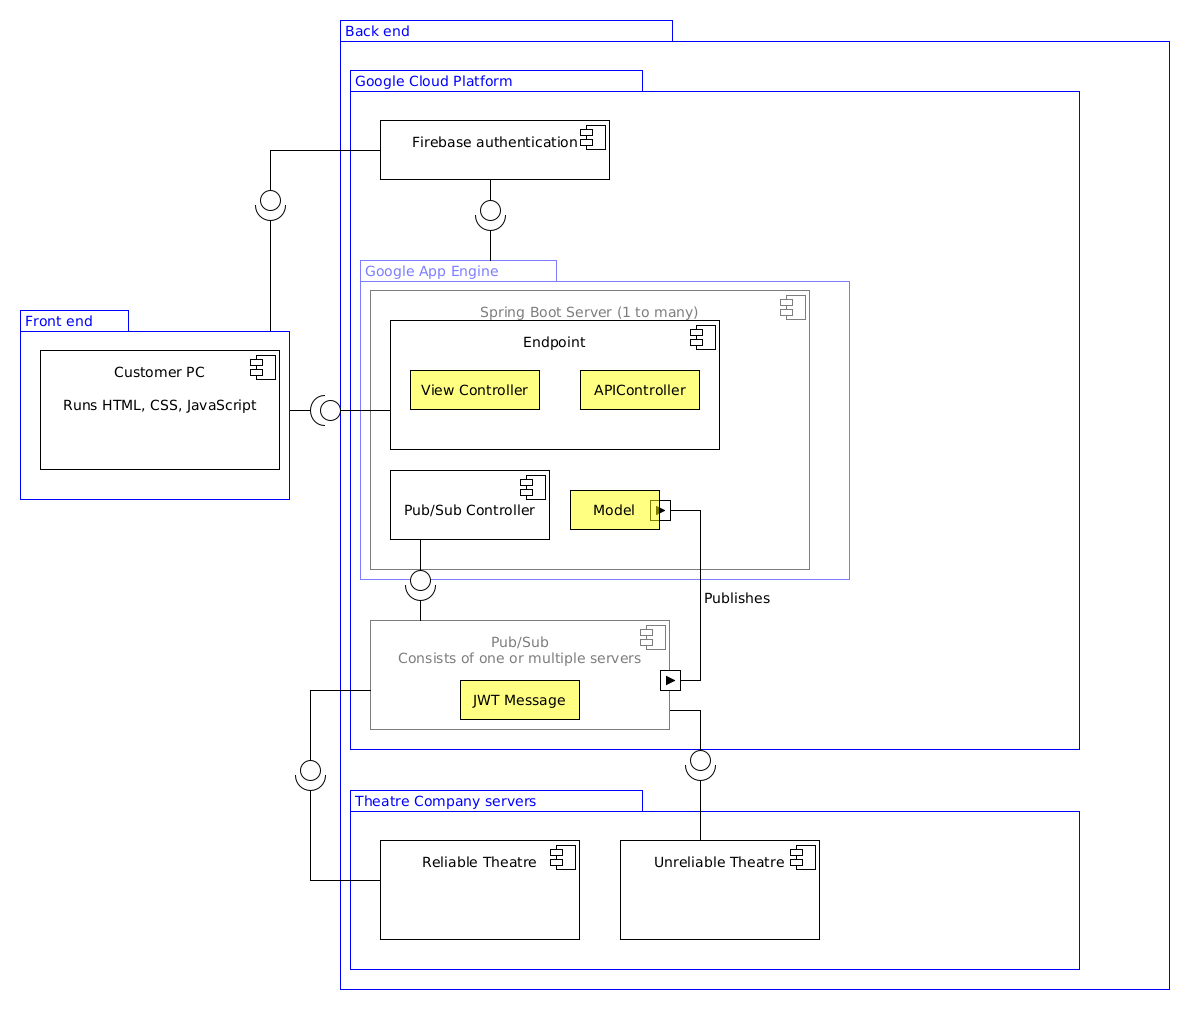
\includegraphics[width=\linewidth]{../diagrams/ComponentDiagram}
		\end{center}
	\caption{Component diagram of part I of the project.}
	\label{fig:component}
	\end{figure}

	
\end{document}